\chapter{Progettazione}
\label{cap:progettazione}

\intro{In questo capitolo verrà illustrata la fase di progettazione del prodotto, partendo dalla realizzazione di un mockup, passando per la definizione dell'architettura e le tecnologie da utilizzare.}\\

\section{Mockup}
\label{sec:mockup}

Il primo passo per la progettazione dell'applicazione è stato quello di realizzare un \gls{mockup}\glsoccur con lo scopo di definirne il più dettagliatamente possibile l'interfaccia grafica: il numero di viste necessarie, la loro struttura, i componenti grafici e la loro disposizione, la \emph{palette} dei colori, come l'utente interagirà con l'applicazione e come questa dovrà rispondere a tali interazioni, simulabili attraverso un prototipo. Infatti, per l'implementazione della \gls{uig}\glsoccur si è rivelato essere di notevole utilità, in quanto ha reso più semplice e veloce la realizzazione di quest'ultima, avendo compreso a priori come questa dovesse essere strutturata.\\
Inoltre il \gls{mockup} è stato utilizzato per definire le funzionalità che l'applicazione deve offrire, in modo da avere un'idea più chiara di come queste debbano essere implementate e, infine, come è stato menzionato nella sezione \ref{subsec:variazione-pianificazione}, è stato indispensabile per la fase di \emph{analisi dei requisiti} .\\ 
Si specifica che nel corso della fase di implementazione sono state apportate delle modifiche all'interfaccia grafica per migliorarne l'usabilità, mantenendo però invariata la struttura generale dell'applicazione e prestando particolare attenzione all'esperienza utente, in modo da rendere l'utilizzo dell'applicazione, in mobilità, il più semplice e intuitivo possibile.\\
|| FORSE, HA SENSO METTERE IN CONFRONTO IL MOCKUP E REALE UI ? ||\\
Di seguito dunque vengono presentate le schermate che compongono il mockup dell'applicazione, con una breve descrizione riguardanti le funzionalità che esse offrono e i componenti grafici che la compongono, con lo scopo di rendere più chiara la loro funzione e il loro utilizzo. 

\subsection{Schermata di login}
\label{subsec:login}


\section{Architettura}
\label{sec:architettura}
% State Management -> RIVERPOD + Diagramma illustrativo
% https://codewithandrea.com/articles/flutter-app-architecture-riverpod-introduction/

% DA CITARE IN BIBLIOGRAFIA E FARNE RIFERIMENTO
La peculiarità di \gls{flutter}\glsoccur è quella di essere un \gls{framework}\glsoccur che permette di sviluppare applicazioni native per diverse piattaforme, come Android, iOS, web e desktop, utilizzando un unico linguaggio di programmazione, riducendo i tempi e i costi di produzione, senza compromettere le prestazioni dell'applicazione.\\
Per comprendere al meglio questa caratteristica è necessario analizzare l'architettura delle applicazioni realizzate in \gls{flutter}\glsoccur, che sono composte dagli elementi illustrati nella figura \ref{fig:architettura-flutter}, tra le quali i principali sono descritti di seguito:
\begin{itemize}
    \item \textbf{Embedder}: fornisce un punto d'ingresso con il sistema operativo ospitante per accedere ai servizi forniti da esso. Questo consente dunque l'esecuzione dell'applicazione su diverse piattaforme e la possibilità di utilizzare librerie per accedere a funzionalità esclusive di determinati sistemi operativi, oppure viceversa, integrare il codice \gls{flutter}\glsoccur in un'applicazione nativa già esistente;
    \item \textbf{Flutter engine}: è il componente centrale che fornisce l'implementazione di basso livello dell'\gls{apig}\glsoccur principale di \gls{flutter}\glsoccur, inclusa la grafica, il layout di testo, operazioni di \emph{I/O}, rete, ecc.;
    \item \textbf{Flutter framework}: componente con il quale lo sviluppatore interagisce attraverso un insieme di librerie, che partendo dal basso sono:
    \begin{itemize}
        \item \textbf{foundation}: fornisce un'astrazione delle funzionalità di animazione, grafica e \gls{gesture}\glsoccur;
        \item \textbf{rendering}: fornisce un'astrazione per gestire il layout. Con questo livello è possibile costruire un albero di oggetti renderizzabili.
        \item \textbf{widget}: ogni oggetto renderizzabile ha una classe corrispondente in questa libreria, definiti appunto \emph{widget}, l'unità fondamentale in \gls{flutter}\glsoccur, che permettono la realizzazione dell'interfaccia grafica;
        \item \textbf{Material e Cupertino}: forniscono un'implementazione di alto livello dei \emph{widget} per la realizzazione di interfacce grafiche seguendo le linee guida di \emph{Material Design} e \emph{Cupertino}, rispettivamente per le piattaforme \emph{Android} e \emph{iOS}.
    \end{itemize}
    \item \textbf{Dart App}: codice sorgente sviluppato dall'utente, contenente i \emph{widget} per l'implementazione della \gls{ui}\glsoccur e la logica dell'applicazione.
\end{itemize}

Inoltre, essendo un \gls{framework}\glsoccur \gls{open-source}\glsoccur, è possibile utilizzare librerie di terze parti, sviluppate dalla community, per aggiungere funzionalità all'applicazione, come ad esempio librerie per la gestione dello stato dell'applicazione, librerie per la gestione delle richieste HTTP, ecc. \\

\begin{figure}[!h] 
    \centering 
    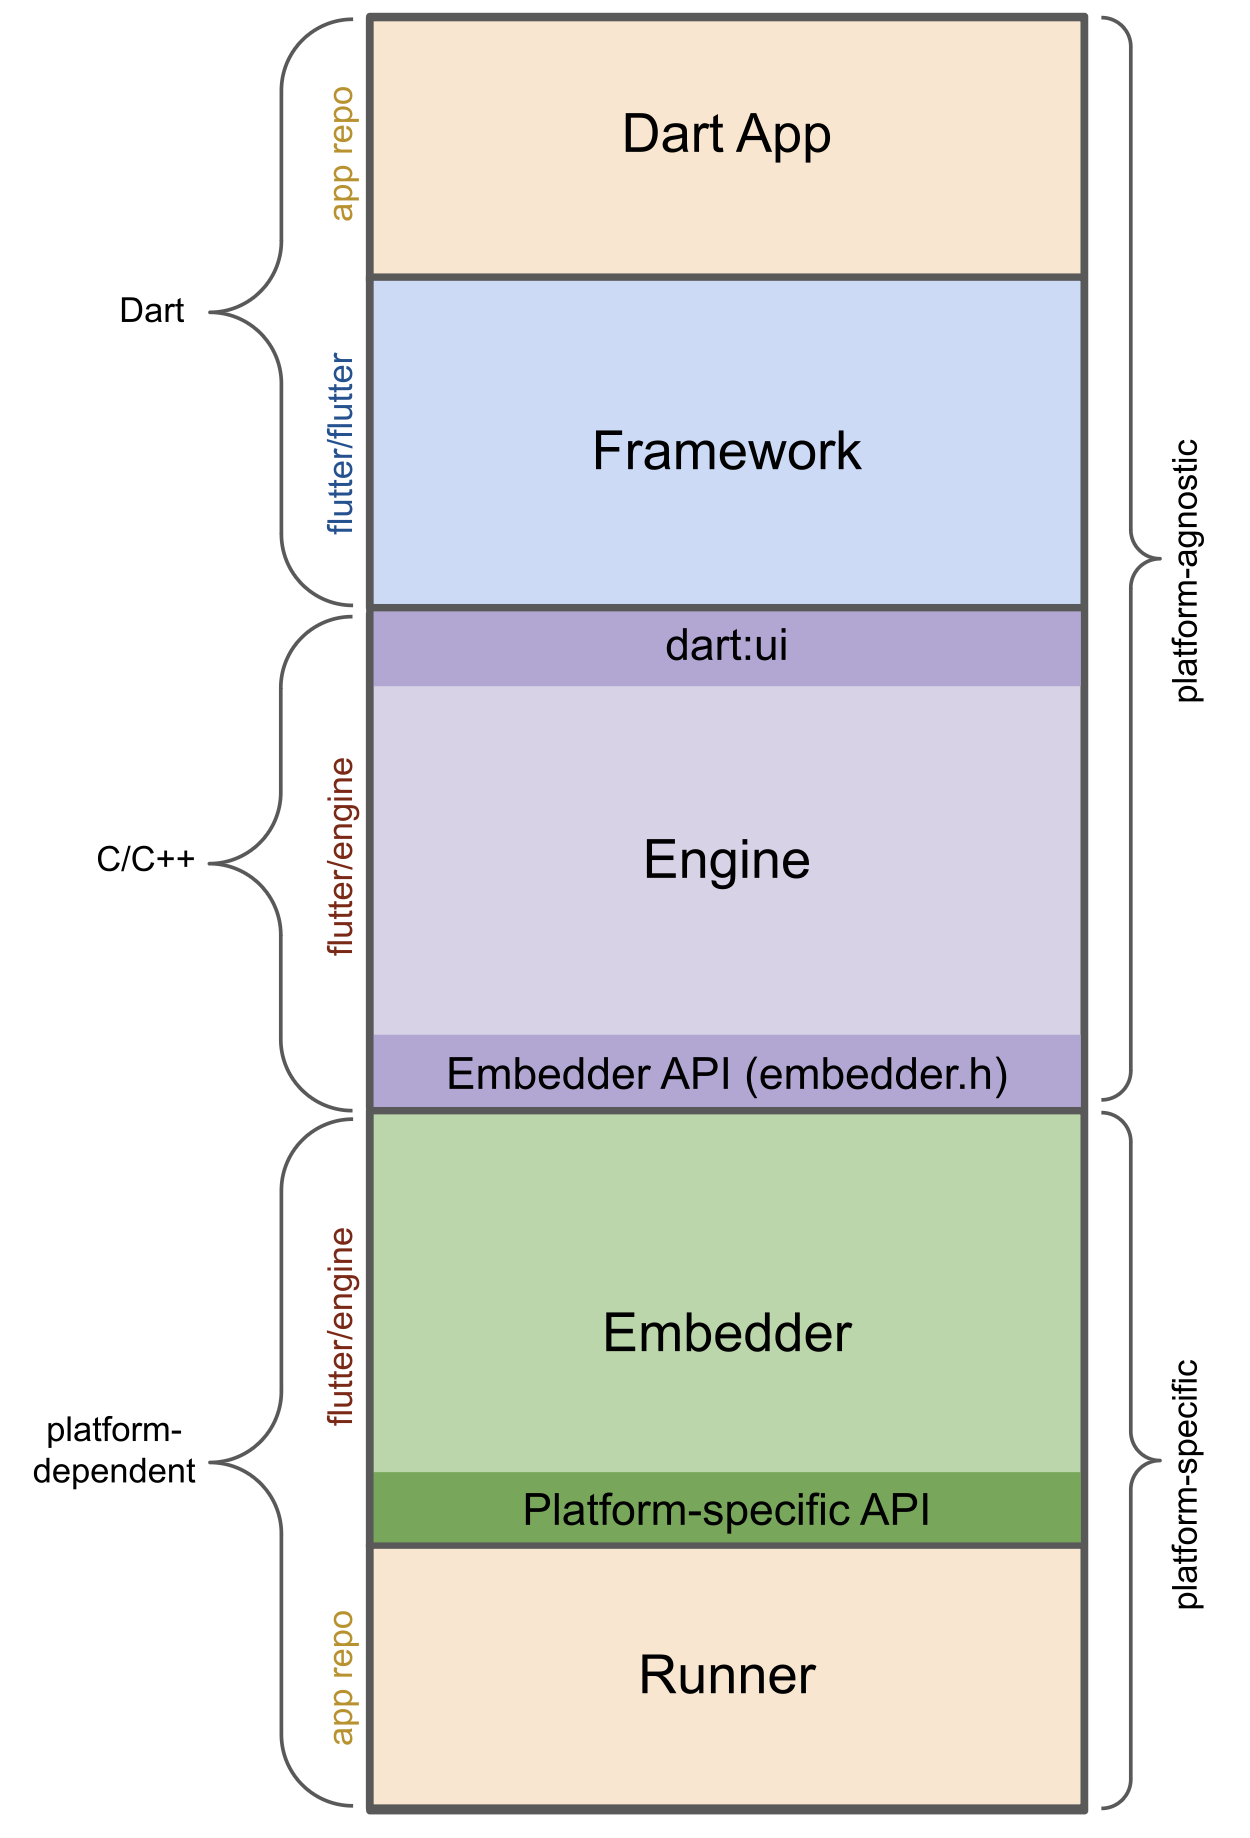
\includegraphics[width=0.4\columnwidth]{images/flutter-app-anatomy.png} 
    \caption{Struttura di un'applicazione in \emph{Flutter}.}
    \label{fig:architettura-flutter}
\end{figure}

Il concetto centrale di \gls{flutter}\glsoccur è quello dei \emph{widget}, oggetti immutabili che descrivono come deve essere visualizzata una parte dell'interfaccia grafica. Questi possono essere di due tipi:
\begin{itemize}
    \item \textbf{StatelessWidget}: non hanno uno stato interno, ovvero non cambiano nel tempo, e sono definiti da un insieme di proprietà, chiamate \emph{proprietà immutabili}, che vengono passate al costruttore del \emph{widget};
    \item \textbf{StatefulWidget}: al contrario, possiedono uno stato interno, e sono definiti da due classi: una che estende \emph{StatefulWidget} e una che estende \emph{State}, quest'ultima rappresenta lo stato interno del \emph{widget}. È un oggetto mutabile, che viene creato quando il \emph{widget} viene inserito nell'albero dei \emph{widget}, e viene distrutto quando viene rimosso dall'albero.
\end{itemize}

Lo stato può essere considerato come \emph{ephemeral} (ing. effimero) o \emph{app state} (ing. stato dell'applicazione). \\
Lo stato \emph{ephemeral} è uno stato che può essere opportunamente confinato all'interno di un singolo \emph{widget} e può essere gestito attraverso la primitiva \lstinline{setState()}, che permette di definire come aggiornarlo.\\
Mentre \emph{app state} è uno stato che viene condiviso tra più \emph{widget} e per la sua gestione, più complessa utilizzando solamente la primitiva sopra citata, esistono diverse librerie di terze parti, ciascuna con le proprie peculiarità a seconda del caso d'uso.\\
\indent La problematica di come gestire lo stato dell'applicazione è definito in gergo \emph{state management}, e dopo un'attenta analisi delle librerie disponibili, si è scelto di utilizzare \href{https://riverpod.dev/}{Riverpod}.\\

\subsection{Riverpod}
\label{subsec:riverpod}
% DA CITARE IN BIBLIOGRAFIA E FARNE RIFERIMENTO

% cos'è
% come funziona
% vantaggi
% svantaggi
% motivazione della scelta
Libreria che semplifica notevolmente lo \emph{state management} e si basa sul concetto di \emph{provider}, evoluto dalla \href{https://pub.dev/packages/provider}{libreria} da cui deriva.\\
A differenza di \emph{InheritedWidget} che permette di condividere lo stato tra più widget, il concetto fondamentale su cui si sono basate queste librerie, \emph{provider}, che ne è una reimplementazione, è indipendente dai \emph{widget}, in quanto è dichiarato a livello globale e può essere richiamato ovunque.\\
Inoltre evita di aggiornare l'interfaccia grafica, ovvero di richiamare il metodo \lstinline{build()} di un \emph{widget} quando non è necessario, poichè è un'operazione costosa.

Un \emph{provider} è un oggetto che può essere letto da un \emph{widget} e che può essere utilizzato per ottenere un valore, che può essere un oggetto o una funzione.\\

\section{Struttura del progetto}
\label{sec:struttura-progetto}
% Struttura del progetto: cartelle, file, ecc. -> LAYER FIRST

% \section{Diagrammi UML}
% \label{sec:uml}
% dove inserirli?
% UML -> Diagrammi delle classi

% \subsubsection{Namespace 1} %**************************
% Descrizione namespace 1.

% \begin{namespacedesc}
%     \classdesc{Classe 1}{Descrizione classe 1}
%     \classdesc{Classe 2}{Descrizione classe 2}
% \end{namespacedesc}

\section{Tecnologie e strumenti}
\label{sec:tecnologie-strumenti}
% SEGUI ISSUE #4 E #5 PER LA STESURA DI QUESTA SEZIONE
Di seguito viene data una panoramica delle tecnologie e strumenti utilizzati.

Per fare ciò è stato utilizzato il software \href{https://www.figma.com/}{Figma}, che permette di creare interfacce grafiche per applicazioni web e mobile.\\

\subsection*{Tecnologia 1}
Descrizione Tecnologia 1.

\subsection*{Tecnologia 2}
Descrizione Tecnologia 2